\documentclass[8pt,twocolumn,a4paper]{article}
\usepackage{amssymb, amsmath,graphicx,soul,color}
\usepackage[affil-it]{authblk}


\newcommand*{\eg}{e.g. }
\newcommand*{\ie}{i.e. }



\begin{document}

\author{Aldosary, Buthainah\\
\texttt{aldosa@encs.concordia.ca}}
\affil{Concordia University\\
 Montreal, Canada}

\date{}
\title{Software Complexities: Do System and Change Complexity Relate?}




\maketitle
\section{Introduction}

The complexity of a change can be very different from the complexity of the
files or system that contain a change (\eg, a change to many simple files
might be as complex as a change to one difficult file). Change complexity is
related to, ``how hard is it to understand and review a change" vs system
complexity, which measures for example, "how hard is it to understand and
potentially modify the system". 

Traditional complexity measures (\eg McCabe) are normed on or require a whole
file or system and were not designed to measure the complexity of changes and
code fragments. The goal of this paper is to evaluate which measures are the
best indicators of the complexity the changes to an evolving system. 


\textbf{We have the following research questions:}

\begin{enumerate}

\item Does the difference of traditional complexity measures before and after a change correlate with change complexity measures?

\item Does the weighted sum of change complexity measures up to a version correlated with the traditional complexity measures at that version? 

\end{enumerate}

\section{Background and Measures}

\subsection{Traditional Complexity Measures}
{\bf{\emph{Metrics Related to Lines of Code}}}
\newline
\begin{enumerate}

\item{\bf{Source Line of Code(SLOC): }} To define SLOC we use the definition given by Conte [Conte 1986]:
A line of code is any line of program text that is not a comment or blank line, regardless of the
number of statements or fragments of statements on the line. This specifically includes all lines containing program headers, declarations, and executable and non-executable statements.

\item{\bf{Lines of Code (LOC): }} Lines of code refers to the total number of lines in each source code file including comments and blank lines. It is a straightforward measure and can be calculated using many available tools.


\item{\bf{BLANK: }}Blank is a count of the number of blank lines.

\item{\bf{COM.L: }}Number of lines that are exclusively comments (no code).

\item{\bf{COM.N: }} Number of comments in the file (a comment can be multiline).
\end{enumerate}


{\bf{\emph{Metrics Related to Complexity}}}
\newline

{\bf{McCabe's Cyclomatic Complexity}}\newline

McCabe’s Cyclomatic complexity is one of the earliest complexity measures developed by Thomas J. McCabe in 1976. It directly measures the number of linearly independent paths through a program's source code. Any program can be represented as a graph with the simplest element being a flat series of statements with no conditions, loops or branches. [1] For a graph $G$ with $n$ vertices, $e$ edges and $p$ exit points, the complexity $v$ is defined as follows:

\begin{equation}
v(G)=e-n+2p
\end{equation}

It is worth mentioning that the minimum value for the cyclomatic complexity metric is 1, which corresponds to the flat series of statements with no bifurcations or loops. Every additional region in the flow graph would increase the Cyclomatic complexity by one unit.
\begin{enumerate}
\item{\bf{ (TOTCY)}}: Total McCabe's cyclomatic complexity (sum of all functions)
\item{\bf{MAXCY: }} Maximum McCabe’s cyclomatic complexity. (between all functions).

\item{\bf{MINCY: }} Minimum McCabe’s cyclomatic complexity.
\item{\bf{AVGCY: }} Average McCabe’s cyclomatic complexity.
\item{\bf{MEDCY: }} Median McCabe’s cyclomatic complexity.

{\bf{Halstead's Complexity Measures}}

Halstead’s complexity metrics rely on the assumption that programs should be viewed as expressions of languages both programming and written. It relies on the premise that there are mathematically sound relationships among the number of variables, the complexity of the code and the type of programming language statements used.

\item{\bf{H.LEN: }}Halstead’s length.
\item{\bf{H.VOL: }}Halstead's volume.

\item{\bf{H.LEVEL: }}Halstead’s level.

\item{\bf{H MEN.D: }}Halstead’s number of mental discriminations.



\end{enumerate}

\subsection{\hl{Change Complexity Measures}}


Each change is calcuated on the difference between two versions of a file.
%
All of our measures are based upon the premise that changes that are farther
from each other or involve multiple entities are more complex than those closer
together involving fewer entities. 
%
In total, we measure change complexity in seven ways:

\begin{itemize}

\item The churn or change size, 

\item The number of modified files per commit,

\item The number of diffs per commit, 

\item The number of and distance between contiguous change blocks within a diff
(\ie hunks), 

\item The directory distance between files, and 

\item The depth of indentation of a change. 

\end{itemize}

%
Since the goal of each measure is the same, to assess the complexity of a
change, we expect some of our measures to be highly correlated. 
%we want the simpliest most parsimonious measures. 
In the interest of parsimony, we will select the simplest set of measures that adequately captures change complexity. 

{\bf Files and diffs:} we count the number of files contained in a commit. The more files that change, the larger the affect proportion of the system. Commits with a large number of files will likely be difficult to understand. 

{\bf Change blocks:} we measure the number of contiguous change blocks, or
hunks, and the distance between these blocks in a modified file and sum them
across the entire review.  Contiguous changes  are likely easier to review than
changes that are far apart and that are potentially in multiple functions
within a file.  

{\bf Directory distance:} we measure the directory distance between the files
in a commit. The premise for this measure is that files that perform similar
functions are typically closer in the directory hierarchy than files that
perform dissimilar functions~\cite{Bowman1999ICSE}, thus the directory
structure loosely mirrors the system architecture~\cite{RigbySubTOSEM}. The
distance of two files in the same directory have a distance of zero, while the
distance for files in different directories is the number of directories
between the two files in the directory hierarchy.  We expect that changes that
involve files that are far apart will crosscut the functionality of a system
and be more complex to review.

{\bf Indentation:} Hindle \cite{Hindle2008ICPC} created a complexity
measure that can be used to measure the complexity of the entire system or of a
change by examining the level of indentation on source lines. We calculate
their measure for reviews. They found that the strongest predictors of
complexity were the sum and standard deviation of the indentation of source
lines. 

%TODO weighted number of people who changed a file?

\section{Methodology and Data}


In figure 1 we illustrate a hypothetical system which undergoes numerous changes. The vertical lines represent each version. During each version's development, the change complexity measures are assessed. In between versions, traditional complexity measures are computed. These are denoted by CCM and TCM respectively.

\begin{figure}[h!]
  \centering
 %  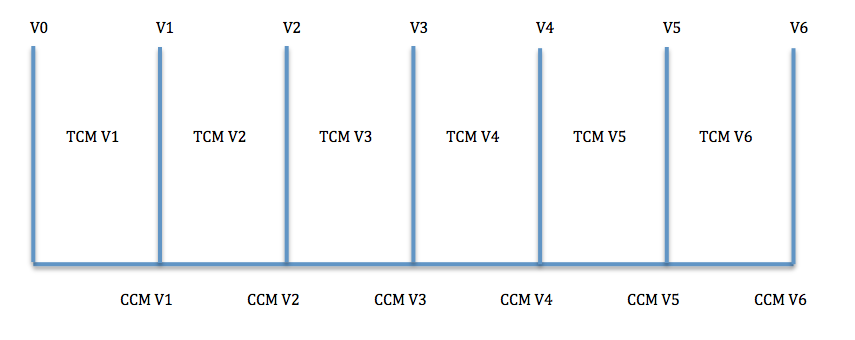
\includegraphics[width=0.5\textwidth]{change_complexity_figure}
   \caption{"Change Complexity vs. Traditional Complexity"}
\end{figure}

\begin{equation}
{{CCM_{v(i)}} = {TCM_{v(i+1)}}-{TCM_{v(i)}}}
\end{equation}

\begin{equation}
{{TCM_{v(i+1)}} = \sum\limits_{i=0}^iCCM_{v(i)}}
\end{equation}
 
\begin{equation}
{{{TCM_{v(i)}} = CCM_{v(i)}}   _{n=1000}}
\end{equation}

\section{Results}

In this section, we compare how correlated each measure is to each other.

\section{Threats to validity}

\section{Conclusion}

Future work: Does McCabe predict anything? Do the change complexity measures do a better job of prediction?

\end{document}
